\chapter{The Prior Problem}

\vspace{1em}
\hfill
\begin{minipage}[c]{0.55\textwidth}
\raggedleft
\small\itshape
The most important questions of life are, for the most part, really only problems of probability.\\[0.5em]
\upshape\footnotesize Pierre-Simon Laplace, \textit{Th\'eorie analytique des probabilit\'es} (1812)
\end{minipage}%
\hspace{0.5em}
\begin{minipage}[c]{0.12\textwidth}
% \includegraphics[width=\textwidth]{figures/ch02_prior.png}
\end{minipage}
\vspace{1.5em}

\noindent The end of Chapter 1 left a hole. Bayes tells you how to update beliefs once you have a prior. It does not tell you what the prior should be.

This hole is not a technical wrinkle. It is structural. To see why, return to the coin.

\section*{Two agents, same data, different conclusions}

Two of your friends, call them Aria and Ben, each receive your report: five heads in a row on a freshly produced coin.

Aria, having read about trick coins, thinks they are quite common in informal contexts. She starts with $P(\text{trick}) = 0.5$. After five heads, by Bayes, her posterior is

$$P(\text{trick} \mid \text{HHHHH}) = \frac{1 \cdot 0.5}{1 \cdot 0.5 + 0.5^5 \cdot 0.5} \approx 0.97.$$

She is quite confident the coin is trick.

Ben, having handled many coins in his life and almost never encountered a trick one, starts with $P(\text{trick}) = 0.001$. After the same five heads,

$$P(\text{trick} \mid \text{HHHHH}) = \frac{1 \cdot 0.001}{1 \cdot 0.001 + 0.5^5 \cdot 0.999} \approx 0.031.$$

He thinks the coin is almost certainly fair; his friend just got lucky.

Same data. Same calculation. Different conclusions. Figure~\ref{fig:priors-diverging} shows the divergence.

\begin{figure}[h]
\centering
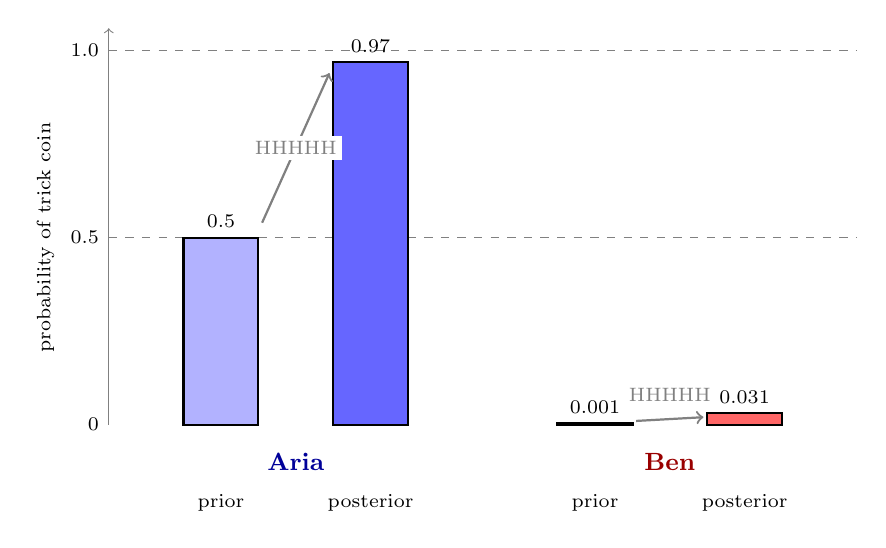
\begin{tikzpicture}[scale=0.95]
  % Y axis
  \draw[->, gray] (0, 0) -- (0, 5.3);
  \node[font=\scriptsize, rotate=90, anchor=south] at (-0.6, 2.5) {probability of trick coin};
  \node[font=\scriptsize, anchor=east] at (0, 0) {0};
  \node[font=\scriptsize, anchor=east] at (0, 2.5) {0.5};
  \node[font=\scriptsize, anchor=east] at (0, 5) {1.0};
  \draw[dashed, gray] (0, 2.5) -- (10, 2.5);
  \draw[dashed, gray] (0, 5) -- (10, 5);

  % Aria's prior (0.5) and posterior (0.97), heights scaled to 2.5 and 4.85
  \fill[blue!30] (1, 0) rectangle (2, 2.5);
  \draw[thick] (1, 0) rectangle (2, 2.5);
  \node[font=\scriptsize, anchor=south] at (1.5, 2.5) {0.5};

  \fill[blue!60] (3, 0) rectangle (4, 4.85);
  \draw[thick] (3, 0) rectangle (4, 4.85);
  \node[font=\scriptsize, anchor=south] at (3.5, 4.85) {0.97};

  \draw[->, gray, thick] (2.05, 2.7) -- (2.95, 4.7);
  \node[font=\scriptsize, gray, fill=white, inner sep=2pt] at (2.5, 3.7) {HHHHH};

  \node[font=\small\bfseries, blue!60!black] at (2.5, -0.5) {Aria};
  \node[font=\scriptsize, anchor=north] at (1.5, -0.8) {prior};
  \node[font=\scriptsize, anchor=north] at (3.5, -0.8) {posterior};

  % Ben's prior (0.001) and posterior (0.031), heights 0.005 and 0.155
  \fill[red!30] (6, 0) rectangle (7, 0.025);
  \draw[thick] (6, 0) rectangle (7, 0.025);
  \node[font=\scriptsize, anchor=south] at (6.5, 0.025) {0.001};

  \fill[red!60] (8, 0) rectangle (9, 0.155);
  \draw[thick] (8, 0) rectangle (9, 0.155);
  \node[font=\scriptsize, anchor=south] at (8.5, 0.155) {0.031};

  \draw[->, gray, thick] (7.05, 0.05) -- (7.95, 0.1);
  \node[font=\scriptsize, gray] at (7.5, 0.4) {HHHHH};

  \node[font=\small\bfseries, red!60!black] at (7.5, -0.5) {Ben};
  \node[font=\scriptsize, anchor=north] at (6.5, -0.8) {prior};
  \node[font=\scriptsize, anchor=north] at (8.5, -0.8) {posterior};

\end{tikzpicture}
\caption{Two reasonable agents, same data, different conclusions. Aria's prior is $0.5$; after HHHHH she lands at $0.97$. Ben's prior is $0.001$; after the same HHHHH he lands at $0.031$. Both use Bayes correctly. The disagreement is downstream of the prior, where Bayes itself has no view.}
\label{fig:priors-diverging}
\end{figure}

Neither is making a mathematical mistake. Both are using Bayes correctly. The disagreement is downstream of the prior, and Bayes itself has nothing to say about who is right.

This is not a fringe case. The same structure appears whenever real agents reason about the world. Doctors interpreting the same test results often disagree because their priors differ. Forecasters give different probabilities for the same weather pattern. Investors looking at the same balance sheet draw different conclusions. In each case the data is shared and the calculation is sound; the prior is doing the work that drives the disagreement.

\section*{The regress}

You might think: fine, the prior is subjective, but it comes from somewhere. From experience, from training, from the next layer of beliefs.

This is correct. It does not solve the problem; it moves it.

If your prior over "is this coin trick" comes from past experience with coins, that past experience was itself processed by some belief-updating mechanism. Presumably Bayes. So your prior over coins is a posterior over coins, derived from earlier data.

Which required an earlier prior over coins.

That earlier prior came from where? From earlier experience, processed by earlier updating. Which required an even earlier prior. Figure~\ref{fig:prior-regress} draws the regress.

\begin{figure}[h]
\centering
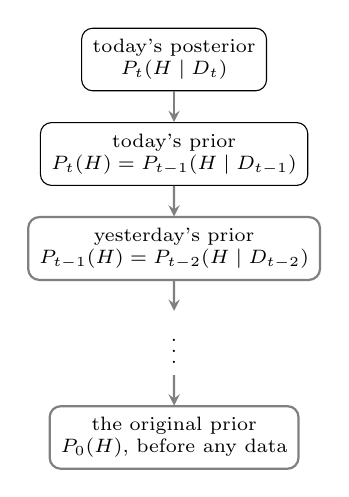
\begin{tikzpicture}[
  every node/.style={align=center, font=\scriptsize, draw, rounded corners, inner sep=4pt},
  level distance=1.2cm,
  edge from parent/.style={draw, ->, >=stealth, thick, gray}
]
  \node {today's posterior\\$P_t(H \mid D_t)$}
    child {node {today's prior\\$P_t(H) = P_{t-1}(H \mid D_{t-1})$}
      child {node {yesterday's prior\\$P_{t-1}(H) = P_{t-2}(H \mid D_{t-2})$}
        child {node[draw=none, fill=none] {\vdots}
          child {node {the original prior\\$P_0(H)$, before any data}}
        }
      }
    };
\end{tikzpicture}
\caption{The prior regress. Every prior is a posterior from an earlier round of Bayesian updating, which required its own prior, which was itself a posterior from an even earlier round. The regress terminates at the original prior $P_0(H)$, the agent's belief before any data has arrived. That original prior is what is at stake.}
\label{fig:prior-regress}
\end{figure}

The regress goes back as far as you take it. Eventually you reach the prior you started with, before any data. The agent's a priori belief, prior to all experience.

That prior is what is at stake. Everything downstream depends on it.

The regress is uncomfortable because it suggests there is no starting point that is not itself a choice. Every belief, traced back far enough, depends on some commitment that was not derived from anything.

\section*{Conventional answers, and why they do not finish the job}

The literature has not been silent. Several proposals exist for how to assign priors when no data has arrived. Each is reasonable in its way; none closes the hole.

\subsection*{Laplace's principle of insufficient reason}

If you know nothing about a situation, treat all outcomes as equally likely. For the coin: if you have no information, give each hypothesis probability one half.

The principle is appealing. It is also fragile. The "equally likely outcomes" depend on how you carve up the possibilities. For the coin you could say: trick or fair, fifty-fifty. Or you could say: the bias parameter of the coin lies somewhere in $[0, 1]$, treat all values equally likely. These two priors give different conclusions. Both seem to express "I know nothing."

The principle works when the partition is natural. When the partition is part of the question, the principle assumes the answer.

\subsection*{Maximum entropy}

A more refined version of the same intuition. Among all priors consistent with what you know, choose the one with maximum entropy: the one that adds the least information beyond your constraints.

Maximum entropy is mathematically clean and has many useful applications. It is also relative to a choice of measure on the space of hypotheses. Different measures give different maximum-entropy priors. The principle is good once you have committed to how to describe the hypotheses; it does not tell you how to describe them.

\subsection*{Expert elicitation}

If you do not know the prior, ask an expert. The expert's belief, calibrated against their experience, becomes your prior.

This works in many applied settings. It does not address the foundational problem. The expert had to get their prior from somewhere too. And different experts disagree.

\subsection*{Empirical Bayes}

Use the data itself to estimate the prior, then update with the rest of the data.

This is a working procedure with real successes. It is not a foundational answer. It uses the data twice, which is fine for engineering and not what we want when asking where the procedure's structure comes from.

\section*{What the standard treatment concludes}

For two and a half centuries, the consensus on the prior problem was: priors are subjective. They reflect agent-specific commitments that no general principle pins down. Different reasonable agents may end with different posteriors, and there is no principled way to declare one of them right.

This is honest and unsatisfying. It tells you Bayes is the right calculus and then leaves the choice of starting point to taste.

For many practical questions, this is acceptable. Agents with reasonable priors and enough data converge. The disagreement washes out. In the long run, what you started with matters less than what you have seen.

But there is a question the standard treatment cannot answer. Imagine a brand-new agent with no past experience, facing the entire universe. There is no past data to lean on. The agent has to start somewhere. Is there a principled starting point?

Or take two agents arguing about a hypothesis with limited data, and the data is not yet enough for their priors to wash out. Which prior is more defensible?

Or take a situation where the data is sparse and the instances differ. (Most situations.) The prior is doing real work in the conclusion. Whose prior is correct?

The standard treatment says: nobody's, in the foundational sense. Pick what is convenient.

This is not a satisfying place to end. The reader who has followed Chapter 1 saw that Bayes is the unique calculus of consistent belief. The reader who follows this chapter sees that the calculus rests on a choice the calculus cannot itself defend.

\section*{A different question}

The next chapter takes a different approach. Instead of asking "how do I assign probabilities to hypotheses I have not seen yet," it asks "how do I assign probabilities to descriptions."

This sounds like a sideways move. It is. The sideways move turns out to close the gap.

The bridge: shorter descriptions can be made more probable than longer ones in a way that is precise and does not depend on choosing a partition or a measure. The bridge is built on prefix-free codes, which Chapter 3 introduces. The result is a principle for assigning priors that has no arbitrary choices to dispute about.

Whether this principle is the right one, and whether it does what we want, are questions Chapter 4 takes up. For now: the hole in Bayes is real, the standard answers do not close it, and there is a different way to think about the problem that has been gathering force since the 1960s.

That is where the book is going.
